\hfill \break
\justifying
El Método en V define un procedimiento para el desarrollo de productos para las TIC, siendo importante mencionar que suele ser un estándar para los proyectos de la Administración Federal alemana y defensa.
Se trata de un modelo rígido y con una gran cantidad de iteraciones siendo similar al modelo de cascada.

\hfill \break
\justifying
El nombre lo toma de su estructura gráfica que suele asemejarse a una letra V, dividiéndose por su parte izquierda en las actividades que descomponen las necesidades y la creación de las especificaciones del sistema. En su parte derecha, se representa la integración de las piezas y su verificación.

\hfill \break
\justifying
La implementación de este tipo de modelo aporta una serie de ventajas que son importantes como objetivos a alcanzar en el proyecto. Este modelo aporta una mejora y garantia de la calidad gracias a las medidas de control de calidad firmemente integradas.
También minimiza los riesgos del proyecto, permitiendo una detección temprana de las desviaciones y riesgos para la mejora de la gestión de los procesos. Otra gran ventaja es la reducción de los gastos totales durante el proyecto y sistema de ciclo de vida, consiguiendose gracias al procesamiento transparente a lo largo de todo el ciclo del producto.

\hfill \break
\justifying
Aun con todas estas ventajas este modelo puede ser poco flexible a cambios durante el desarrollo, promoviendo un curso lineal del proyecto, sin embargo si el modelo es entendido y se utiliza correctamente es posible utilizar el modelo V para el desarrollo agil.

\hfill \break
\justifying
El modelo V define el curso del proyecto en fases individuales cada vez más detalladas(Definición del proyecto):
\begin{itemize}
	\item \textbf{Fase de especificaciones}: Prevé un análisis de las especificaciones del sistema a grandes rasgos
	\item \textbf{Fase funcional}: Se complementa el proyecto con requisitos funcionales y no funcionales para la arquitectura del sistema
	\item \textbf{Fase de diseño}: Se planifican los componentes y las interfaces con un diseño detallado
	\item \textbf{Codificación}: Completadas estas fases inicial el desarrollo de la arquitectura en software
\end{itemize}

\hfill \break
\justifying
En la corriente de pruebas del lado derecho(Prueba e integración del proyecto) consiste de:
\begin{itemize}
	\item \textbf{Pruebas unitarias}: Permiten declarar que un módulo esta listo y terminado: Lógica de módulos(caja blanca), Funciones(Caja negra)
	\item \textbf{Pruebas de integración}: Implican una progresión ordenada de pruebas que van desde los componentes o módulos y que culmina en el sistema completo
	\item \textbf{Pruebas de Sistema}: Se verifica el cumplimiento de los objetivos y se validan los desajustes entre el software y los requisitos planteados
	\item \textbf{Pruebas de Aceptación}: El usuario final comprueba que el sistema hace lo especificado en el contrato
\end{itemize}


\begin{figure}[!h]
	\centering
	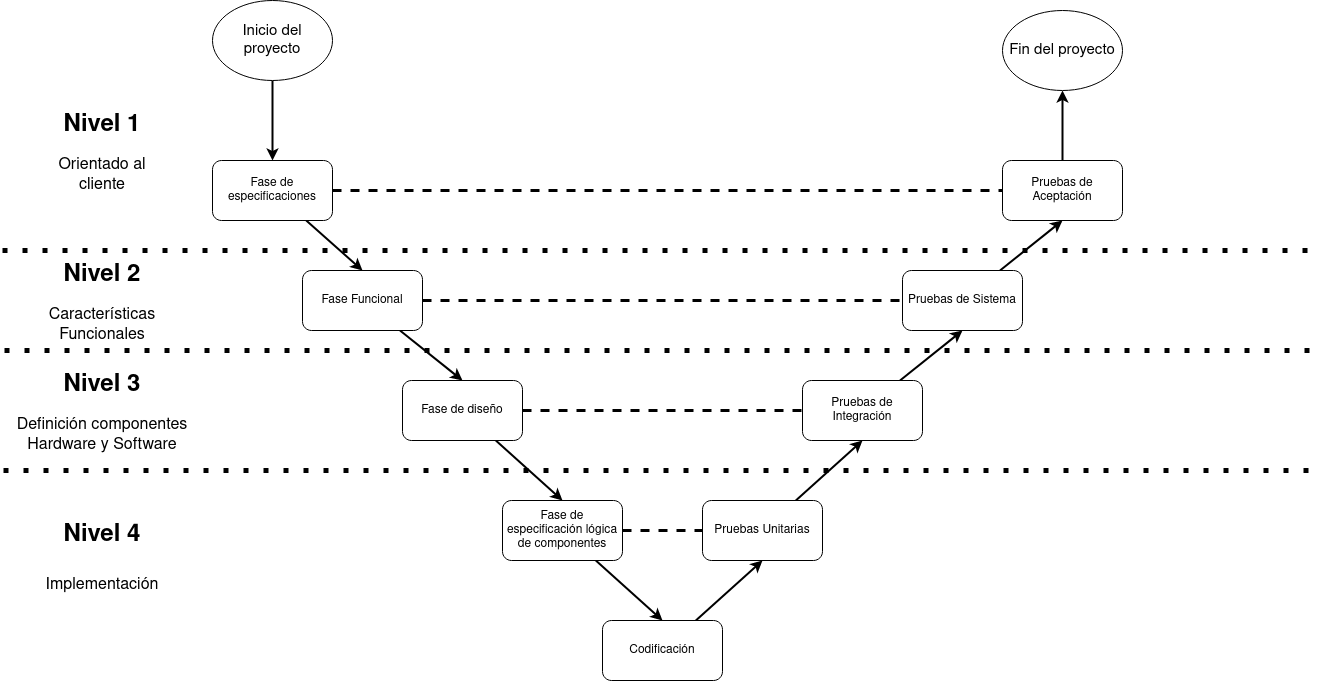
\includegraphics[width=16cm]{Imagenes/Modelo_V.png}
	\caption{Diagrama mostrando las fases del Modelo V}
	\label{Modelo_V}
\end{figure}